\section{(0,2)序列采样器}\label{sec:(0,2)序列采样器}
\begin{remark}
    本节含有高级内容,第一次阅读时可以跳过。
\end{remark}

另一个生成高质量样本的方法是利用某些低偏差序列的显著性质
即允许我们满足两个想要的样本性质(其中仅一个用\refvar{StratifiedSampler}{}满足了):
它们为图像样本的一个像素值生成样本向量使得每个像素样本的样本值都彼此间分布良好,
同时该像素中所有像素样本的样本值集合也整体上分布良好。

该序列使用Sobol\footnote{\protect\refsec{Sobol采样器}的\refvar{SobolSampler}{}使用了
    Sobol序列的所有维度。}推导出的低偏差序列的前两维。
该序列是一种特殊类型的低偏差序列,称为$(0,2)$序列。
$(0,2)$序列以非常常规的方式分层。例如,$(0,2)$序列中的前16个样本
满足来自\refsec{分层采样}中分层采样的分层约束,
意味着每个范围为$\displaystyle\left(\frac{1}{4},\frac{1}{4}\right)$的矩形中只存在一个样本。
然而它们还满足拉丁超立方约束,即在每个范围为$\displaystyle\left(\frac{1}{16},1\right)$和
$\displaystyle\left(1,\frac{1}{16}\right)$的矩形中只有一个样本。
此外,在每个范围为$\displaystyle\left(\frac{1}{2},\frac{1}{8}\right)$和
$\displaystyle\left(\frac{1}{8},\frac{1}{2}\right)$的矩形中只有一个样本。

\reffig{7.28}展示了划分域的所有可能,其中$(0,2)$序列前16个样本都满足分层性质。
从该模式中获取的每组含16个样本的后续序列也都满足这些分布性质。
\begin{figure}[htbp]
    \centering
    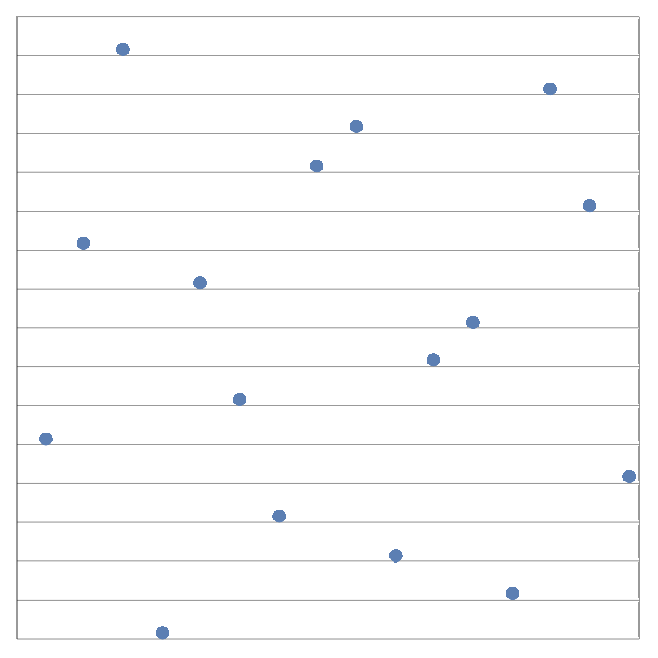
\includegraphics[width=0.49\linewidth]{chap07/elementary1x16.eps}\,
    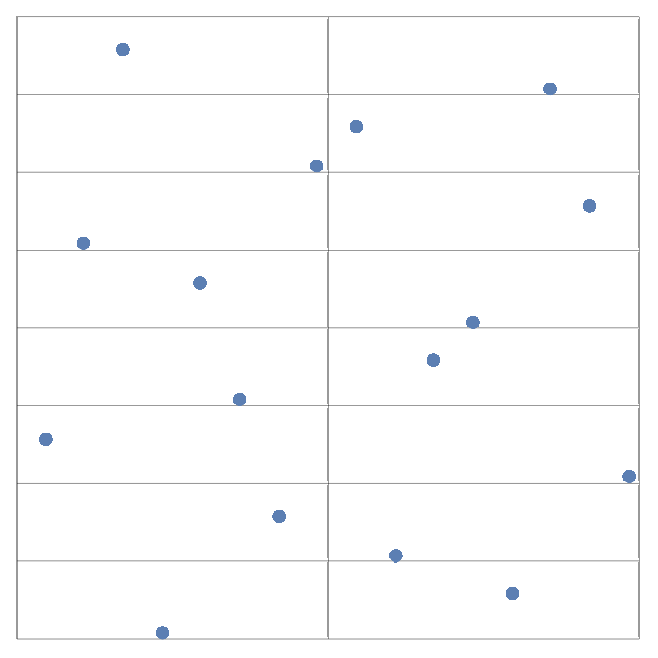
\includegraphics[width=0.49\linewidth]{chap07/elementary2x8.eps}\\
    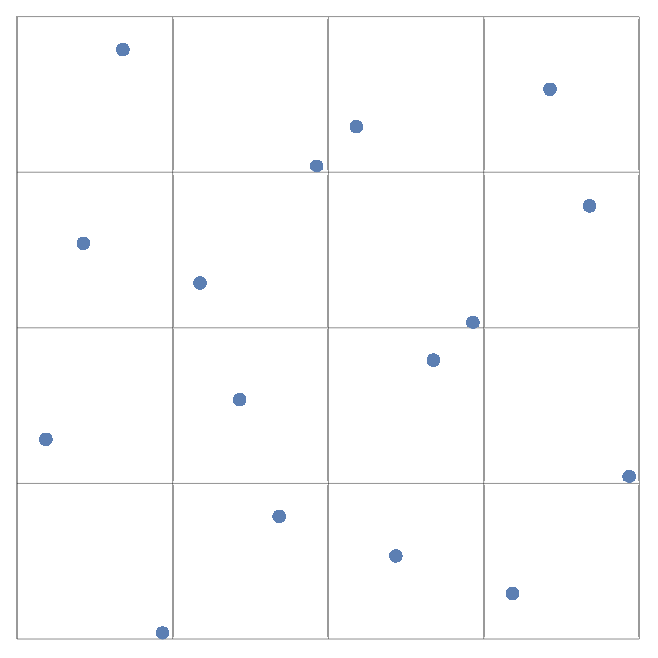
\includegraphics[width=0.49\linewidth]{chap07/elementary4x4.eps}\,
    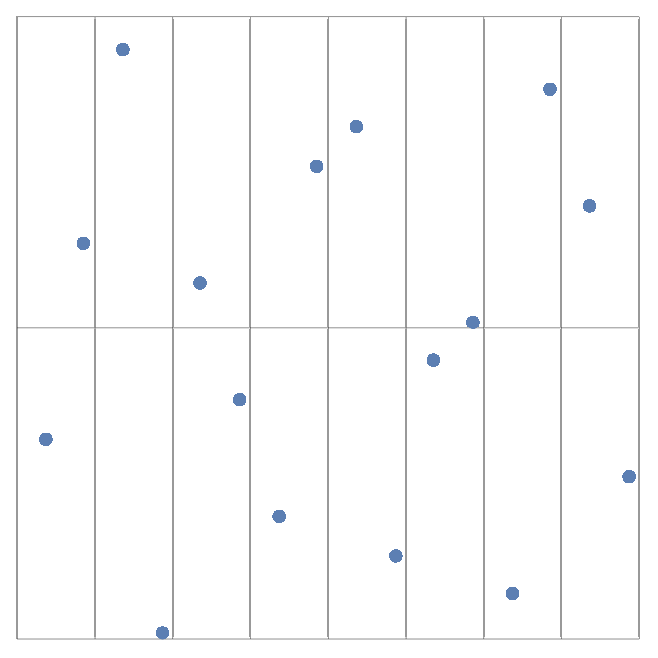
\includegraphics[width=0.49\linewidth]{chap07/elementary8x2.eps}\\
    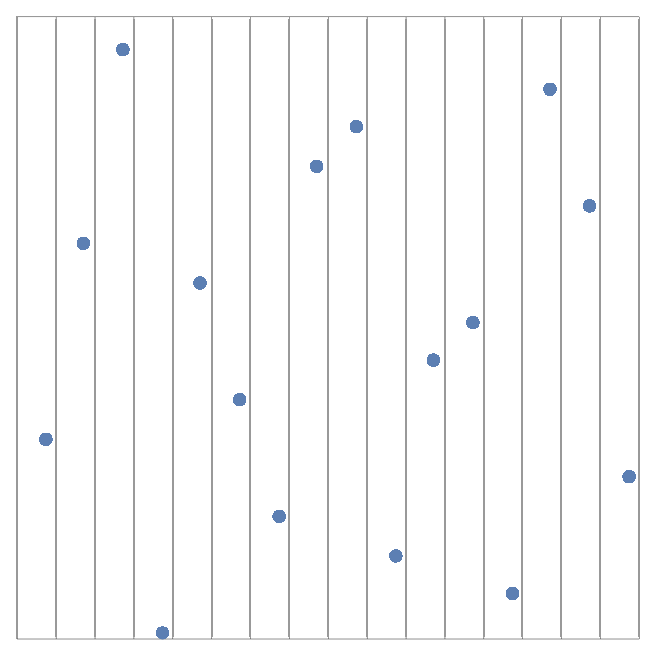
\includegraphics[width=0.49\linewidth]{chap07/elementary16x1.eps}
    \caption{在所有以2为底数的基本区间中都只有单个样本的采样模式。
        它同时满足$4\times4$分层和拉丁超立方约束以及所示的其他两个分层约束。}
    \label{fig:7.28}
\end{figure}

通常任何来自$(0,2)$序列的长为$2^{l_1+l_2}$的序列(其中$l_i$为非负整数)
都满足该一般分层约束。以2为底的两维的\keyindex{基本区间}{elementary interval}{}定义为
\begin{align*}
    E=\left\{\left[\frac{a_1}{2^{l_1}},\frac{a_1+1}{2^{l_1}}\right)\times\left[\frac{a_2}{2^{l_2}},\frac{a_2+1}{2^{l_2}}\right)\right\}\, ,
\end{align*}
其中整数$a_i=0,1,2\ldots,2^{l_i}-1$.
该序列中前$2^{l_1+l_2}$个值中的每一个样本都在相应基本区间中。
此外,后续每$2^{l_1+l_2}$个值构成的集合也满足同样的性质。

现在为了理解怎样把$(0,2)$序列应用于生成2D样本,
考虑有$2\times2$图像样本的像素,每个含$4\times4$个2D样本构成的数组。
依据相应的基本区间集,$(0,2)$序列前$(2\times2)\times(4\times4)=2^6$个值相互之间分布良好。
此外依据其相应的基本区间,前$4\times4=2^4$个样本自己也分布良好,
其后的$2^4$个也是这样,以此类推。因此,我们可以为一个像素的
首个图像样本的$4\times4$数组样本使用前16个$(0,2)$序列样本,
然后下一个图像样本用接下来的16个,以此类推。
结果是分布非常良好的样本点集。

\subsection{用生成矩阵采样}\label{sub:用生成矩阵采样}
比起\refvar{HaltonSampler}{},Sobol序列基于不同的样本点生成机制,
它在各维度上使用了倒根。即使将倒根函数中的整数除法转化为乘法和位移,
高质量高分辨率渲染所需的计算数十亿样本的计算量也会很大。
大部分计算开销来自于在天生是2进制的计算机上执行不以2为底的计算
(考虑代码片\refcode{Compute base-2 radical inverse}{}和模板函数\refvar{RadicalInverseSpecialized}{()}间的差别)。

假设不以2为底的计算有很高开销,自然要尝试开发完全用2进制运算的样本生成算法。
一个这样高效的方法是用\keyindex{生成矩阵}{generator matrix}{},
它允许在相同基中完成所有计算。不像Halton采样器那样在每个维度使用不同基,
它在每个维度使用不同生成矩阵。为每个采样维度精选好矩阵,
就能生成非常好的低偏差分布点。例如,$(0,2)$序列可用两个特定的2进制生成矩阵定义。

为了看看怎样使用生成矩阵,考虑一个$n$位$b$进制数$a$,
其中$a$的第$i$个数字是$d_i(a)$,且我们有个$n\times n$生成矩阵$\bm C$.
则相应样本点$x_a\in[0,1)$定义为
\begin{align}\label{eq:7.9}
    x_a=[b^{-1}\,b^{-2}\, \cdots\,b^{-n}]\left[
        \begin{array}{cccc}
            c_{1,1} & c_{1,2} & \cdots & c_{1,n} \\
            c_{2,1} & \ddots  &        & c_{2,n} \\
            \vdots  &         & \ddots & \vdots  \\
            c_{n,1} & \cdots  & \cdots & c_{n,n}
        \end{array}
        \right]
    \left[
        \begin{array}{c}
            d_1(a) \\
            d_2(a) \\
            \vdots \\
            d_n(a)
        \end{array}
        \right]\, ,
\end{align}
其中的所有运算都在环$\mathsf{Z}_b$中执行(换句话说,所有运算都按模$b$执行)。
当$a$从0变到$b^n-1$时,这一构造给出一共$b^n$个点。
如果该生成矩阵是单位矩阵,则该定义对应于常规的基$b$倒根
(在继续之前,值得你停下来看看\refeq{7.7}与\refeq{7.9}间的联系)。

本节中,我们将只用$b=2$和$n=32$.尽管把$32\times32$矩阵引入样本生成算法
可能看似不是迈向更优性能的一步,但我们最终将看到采样代码可以映射为
以极为高效的方式用少量位运算执行该计算的实现。

迈向高性能的第一步来自我们按2进制处理的事实;
这样$\bm C$的所有元素不是0就是1,
且因此我们可以把矩阵每行或每列表示为一个无符号32位整数。
我们将选择把矩阵的列表示为{\ttfamily uint32\_t};
该抉择得到一个让$d_i$列向量和$\bm C$相乘的非常高效的算法。

现在考虑计算矩阵-向量乘积${\bm C}[d_i(a)]^{\mathrm{T}}$的任务;
利用矩阵-向量乘积的定义,我们有:
\begin{align}\label{eq:7.10}
    \left[
        \begin{array}{cccc}
            c_{1,1} & c_{1,2} & \cdots & c_{1,n} \\
            c_{2,1} & \ddots  &        & c_{2,n} \\
            \vdots  &         & \ddots & \vdots  \\
            c_{n,1} & \cdots  & \cdots & c_{n,n}
        \end{array}
        \right]\left[
        \begin{array}{c}
            d_1(a) \\
            d_2(a) \\
            \vdots \\
            d_n(a)
        \end{array}
        \right]
    =d_1\left[
        \begin{array}{c}
            c_{1,1} \\
            c_{2,1} \\
            \vdots  \\
            c_{n,1}
        \end{array}
        \right]+\cdots+d_n\left[
        \begin{array}{c}
            c_{1,n} \\
            c_{2,n} \\
            \vdots  \\
            c_{n,n}
        \end{array}
        \right]\, .
\end{align}
换句话说,对于$d_i$每个值为1的数字,$\bm C$的对应列应被求和。
该加法反过来可以在$\mathsf{Z}_2$中高效执行:
在该设置下,加法对应于异或运算(考虑两个运算值可能的组合——
0和1——相加$\mod{2}$的结果,并与同样运算值异或后算出的值比较)。
因此,乘法${\bm C}[d_i(a)]^{\mathrm{T}}$只是在$d_i(a)$位为1处
将$\bm C$的第$i$列异或在一起。该计算在函数\refvar{MultiplyGenerator}{()}中实现。
\begin{lstlisting}
`\refcode{Low Discrepancy Inline Functions}{+=}\lastnext{LowDiscrepancyInlineFunctions}`
inline uint32_t `\initvar{MultiplyGenerator}{}`(const uint32_t *C, uint32_t a) {
    uint32_t v = 0;
    for (int i = 0; a != 0; ++i, a >>= 1)
        if (a & 1)
            v ^= C[i];
    return v;
}
\end{lstlisting}

现在回到\refeq{7.9},若我们把积中的列向量
记为$v={\bm C}[d_i(a)]^{\mathrm{T}}$,则考虑向量积
\begin{align}\label{eq:7.11}
    x_a=[2^{-1}\, 2^{-2}\,\cdots\, 2^{-n}]\left[
        \begin{array}{c}
            v_1    \\
            v_2    \\
            \vdots \\
            v_n
        \end{array}
        \right]=\sum\limits_{i=1}^{32}{2^{-i}v_i}\, .
\end{align}
因为$v$的元素存于单个{\ttfamily uint32\_t},其值理解为{\ttfamily uint32\_t}时是
\begin{align*}
    v=v_1+2v_2+\cdots=\sum\limits_{i=1}^{32}{2^{i-1}v_i}\, .
\end{align*}
如果我们翻转{\ttfamily uint32\_t}内的数位顺序,则我们将有值
\begin{align*}
    v'=\sum\limits_{i=1}^{32}{2^{32-i}v_i}\, .
\end{align*}
这是更有用的值:如果我们将该值除以$2^{32}$,则我们得到\refeq{7.11},
即我们要尝试算出的$x_a$.

因此,如果我们取函数\refvar{MultiplyGenerator}{()}的结果,
颠倒返回值的数位顺序(例如用\refvar{ReverseBits32}{()}),
再用该值除以$2^{32}$以计算$[0,1)$中的浮点数,我们就算出了样本值。

为了节约翻转数位的小小开销,我们可以在传入\refvar{MultiplyGenerator}{()}之前
等价地翻转生成矩阵$\bm C$所有列的数位。接下来我们将遵循该约定。

实践中为了让$(0,2)$序列有用,我们还需要能为
每个图像样本生成多个不同的2D样本值集合,
且我们想为每个像素生成不同的样本值。
该问题的一个方法是为每个像素使用从$(0,2)$序列精选的不重叠子序列
\footnote{\refsec{Sobol采样器}的Sobol采样器采用该方法。}。
另一种方法是随机置乱$(0,2)$序列,通过把随机重排应用于原始序列值$b$进制数字
而构建得到新的$(0,2)$序列。

我们将用的置乱方法归功于\citet{10.1111/1467-8659.00706}。
它反复划分与打乱单位方形$[0,1)^2$.
在这两维的每一个中,它都先将该方形对半分再以50\%的概率交换这两半。
然后它再分别对半划分区间$[0,0.5)$和$[0.5,1)$并随机交换其两半。
该过程递归持续直到2进制表示的所有数位都处理完。
仔细设计该过程使其保留点集的低偏差性质;否则$(0,2)$序列的优势会在置乱时流失。
\reffig{7.29}展示了未置乱的$(0,2)$序列及其两个随机置乱的变种。
\begin{figure}[htbp]
    \centering
    \subfloat[]{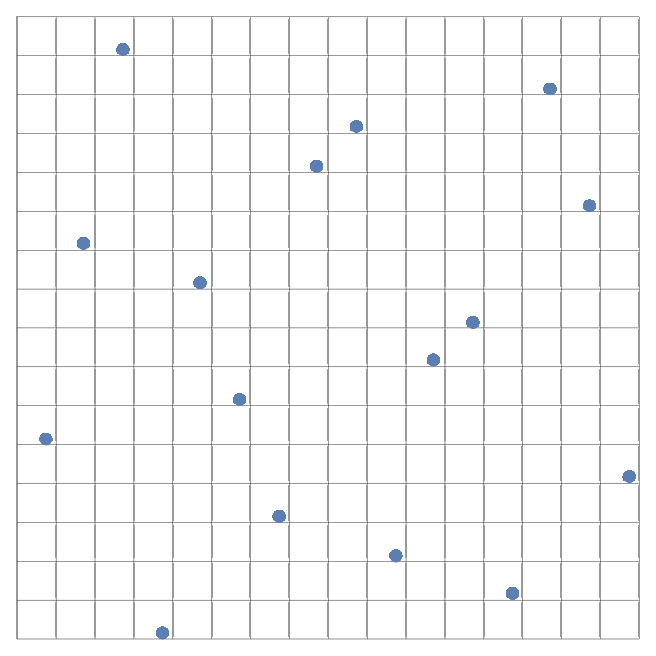
\includegraphics[width=0.3\linewidth]{chap07/02-a.eps}\label{fig:7.29.1}}\quad
    \subfloat[]{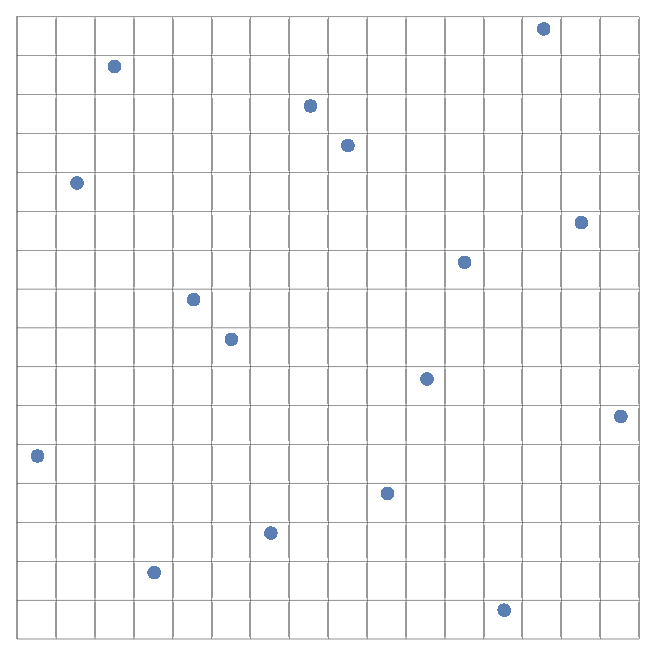
\includegraphics[width=0.3\linewidth]{chap07/02-b.eps}\label{fig:7.29.2}}\quad
    \subfloat[]{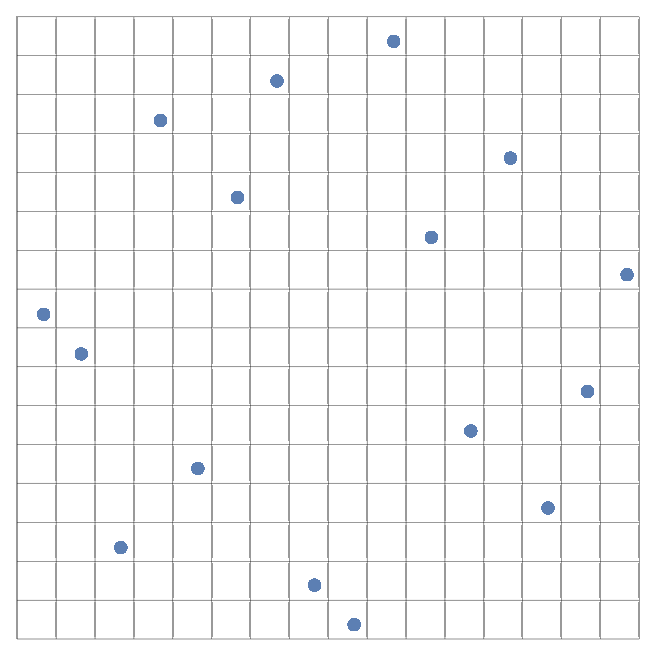
\includegraphics[width=0.3\linewidth]{chap07/02-c.eps}\label{fig:7.29.3}}
    \caption{(a)基于低偏差$(0,2)$序列的采样模式以及(b,c)其两个随机置乱的例子。
        若我们在每个像素中用相同的采样模式,则图像中可能出现伪影,
        而低偏差模式的随机置乱是消除它的高效方法,且仍保留所用点集的低偏差性质。}
    \label{fig:7.29}
\end{figure}

函数\refvar{SampleGeneratorMatrix}{()}将这些片段组合在一起以生成样本值。
\begin{lstlisting}
`\refcode{Low Discrepancy Inline Functions}{+=}\lastnext{LowDiscrepancyInlineFunctions}`
inline `\refvar{Float}{}` `\initvar{SampleGeneratorMatrix}{}`(const uint32_t *C, uint32_t a,
        uint32_t scramble = 0) {
    return (`\refvar{MultiplyGenerator}{}`(C, a) ^ scramble) * 0x1p-32f;
}
\end{lstlisting}

函数\refvar{SampleGeneratorMatrix}{()}已经足够高效,
它每次在运行次数等于值{\ttfamily a}以2为底的对数
的\refvar{MultiplyGenerator}{()}循环中执行少量算数运算。
值得注意的是,通过改变生成样本的顺序、
以\keyindex{格雷码}{Gray code}{}顺序枚举甚至可以做得更好。

用格雷码表示的连续二进制值只相差一位;
\reftab{7.4}的第三列展示了格雷码顺序下的前八个整数。
注意不仅任意一对值之间只有一位改变,
而且在从0起的幂2个即$n$个值中,格雷码枚举了从0到$n-1$的所有值,
只是和平常的顺序不同。
\begin{table}[htbp]
    \centering
    \begin{tabular}{cccc}
        \toprule
        $n$\textbf{(10进制)} & $n$\textbf{(2进制)} & $g(n)$ & \textbf{改变的数位索引} \\
        \midrule
        0                      & 000                   & 000    & n/a                     \\
        1                      & 001                   & 001    & 0                       \\
        2                      & 010                   & 011    & 1                       \\
        3                      & 011                   & 010    & 0                       \\
        4                      & 100                   & 110    & 2                       \\
        5                      & 101                   & 111    & 0                       \\
        6                      & 110                   & 101    & 1                       \\
        7                      & 111                   & 100    & 0                       \\
        \bottomrule
    \end{tabular}
    \caption{格雷码顺序下的前八个整数。每个格雷码值$g(n)$和前一个$g(n-1)$都只有一位不同。
        改变的那位索引由2进制值$n$的尾零个数给出。注意从0起的任意$n$个即幂2个值集合中,
        0到$n-1$间的全部整数都表示了出来,只是和平常的顺序不同。}
    \label{tab:7.4}
\end{table}

可以非常高效地完成计算第$n$个格雷码值。
\begin{lstlisting}
`\refcode{Low Discrepancy Inline Functions}{+=}\lastnext{LowDiscrepancyInlineFunctions}`
inline uint32_t `\initvar{GrayCode}{}`(uint32_t n) {
    return (n >> 1) ^ n;
}
\end{lstlisting}

通过按格雷码顺序枚举样本,我们能极大利用在连续样本间$g(n)$只有一位改变的事实。
假设我们已经为某个索引$a$算出积${\bm C}[d_i(a)]^{\mathrm{T}}=v$:
如果另一个值$a'$和$a$只有一位不同,则我们只需从$v$中加上或减去$\bm C$的一列
以求得$v'={\bm C}[d_i(a')]^{\mathrm{T}}$(回想\refeq{7.10})
\sidenote{译者注:原文将$d_i(a')$误写为$d_I(a')$,已修正。}。
甚至更好的是,加法和减法$\mod{2}$都能用异或执行,
所以需要哪种运算并不重要;我们只需要知道哪一位改变了。
从\reftab{7.4}可以看出,从$g(i)$到$g(i+1)$变化的数位索引由
$i+1$的2进制表示的尾零数目给出。大部分CPU指令集可以在单条指令内数出尾零数量。

综上所述,我们可以用格雷码顺序下的生成矩阵非常高效地生成一系列样本。
\refvar{GrayCodeSample}{()}接收生成矩阵{\ttfamily C},
要生成的样本数量{\ttfamily n},并在{\ttfamily p}所指的内存位置中存储相应样本。
\begin{lstlisting}
`\refcode{Low Discrepancy Inline Functions}{+=}\lastnext{LowDiscrepancyInlineFunctions}`
inline void `\initvar{GrayCodeSample}{}`(const uint32_t *C, uint32_t n,
        uint32_t scramble, Float *p) {
    uint32_t v = scramble;
    for (uint32_t i = 0; i < n; ++i) {
        p[i] = v * 0x1p-32f;  /* 1/2^32 */
        v ^= C[`\refvar{CountTrailingZeros}{}`(i + 1)];
    }
}
\end{lstlisting}

内部循环(省略了循环控制逻辑)的核心x86汇编代码非常简单:
\begin{lstlisting}
    xorps      %xmm1, %xmm1
    cvtsi2ssq  %rax, %xmm1
    mulss      %xmm0, %xmm1
    movss      %xmm1, (%rcx,%rdx,4)
    incq       %rdx
    bsfl       %edx, %eax
    xorl       `\$`31, %eax
    xorl       (%rdi,%rax,4), %esi
\end{lstlisting}

即使不是x86汇编语言的爱好者,也能看出这是生成每个样本值的非常简短的指令序列。

还有生成2D样本的第二版\refvar{GrayCodeSample}{()}(这里没有介绍);
它为每维接收一个生成矩阵并把样本填入{\refvar{Point2f}{}}值的数组。

\subsection{采样器实现}\label{sub:采样器实现02}
\refvar{ZeroTwoSequenceSampler}{}用置乱的$(0,2)$序列
为胶片平面、透镜上的位置以及其他2D样本生成样本,
并用置乱的van der Corput序列生成1D样本。
\begin{lstlisting}
`\initcode{ZeroTwoSequenceSampler Declarations}{=}`
class `\initvar{ZeroTwoSequenceSampler}{}` : public `\refvar{PixelSampler}{}` {
public:
    `\refcode{ZeroTwoSequenceSampler Public Methods}{}`
};
\end{lstlisting}